\documentclass[aspectratio=1610,onlymath]{beamer}
% \documentclass[aspectratio=1610,onlymath,handout]{beamer}

\input{macros-lecture}

\defineTitle{24}{Gödel, Turing und der ganze Rest}{19. Juli 2026}

\begin{document}

\maketitle

\frame{\label{frame_goedel}\begin{center}
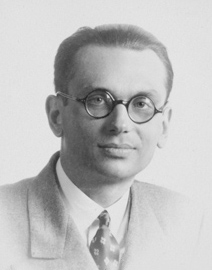
\includegraphics[height=5cm]{images/Goedel.jpg}

\LARGE
Kurt Gödel
\end{center}}

% Goedels Unvollstaendigkeitssaetze (mit vagen Formulierungen), ev. erstmal nur UV1
\begin{frame}\frametitle{Der 1. Gödelsche Unvollständigkeitssatz}

\theobox{\emph{Satz (Gödel, 1931):} Jedes konsistente formale System, in dem eine gewisse Menge elementarer Arithmetik korrekt
dargestellt werden kann, ist unvollständig in Bezug auf die Beweisbarkeit von Sätzen der
elementaren Arithmetik.
}\bigskip

\emph{Relevante Begriffe:}
\begin{itemize}
\item \alert{Formales System:} Ein implementierbares Verfahren, mit dem man Theoreme endlich beweisen kann
\item \alert{Konsistent:} Man kann niemals eine Aussage und ihr Gegenteil beweisen.
\item \alert{Gewisse Menge Arithmetik:} Kodierung konkreter natürlicher Zahlen und deren korrekte Addition, Subtraktion, Multiplikation und Vergleich
\item \alert{Unvollständig:} Es gibt Sätze, die weder bewiesen noch widerlegt werden können
\end{itemize}

\end{frame}

\begin{frame}\frametitle{Beispiele}

\examplebox{\emph{Beispiel:} Natürliche Zahlen und einfache Rechenregeln können mit einer prädikatenlogischen Theorie definiert werden. Mit Resolution kann man daraus korrekte neue Schlüsse ziehen. Laut Gödels erstem Satz kann man auf diese Art aber niemals alle wahren Aussagen der Arithmetik beweisen, außer wenn die Theorie widersprüchlich ist.}

\redalert{Keine prädikatenlogische Theorie kann die elementare Arithmetik vollständig beschreiben.}\pause\bigskip

\examplebox{\emph{Beispiel:} Die moderne Mathematik basiert auf der Mengenlehre von Zermelo-Fraenkel unter Hinzunahme des Auswahlaxioms. Dieses formale System heißt \alert{ZFC}. Es ist klar definiert, was ein korrekter mathematischer Beweis in ZFC ist. Laut Gödels erstem Satz gibt es also wahre Aussagen über elementare Arithmetik, die nicht in ZFC bewiesen werden können.}

\end{frame}

\begin{frame}\frametitle{Gödels 2. Unvollständigkeitssatz}

Gödel kam direkt zu einer weiteren Schlussfolgerung:\medskip

\theobox{\emph{Satz:} Jedes konsistente formale System, in dem eine gewisse Menge elementarer Arithmetik korrekt
dargestellt werden kann, kann nicht seine eigene Konsistenz \\beweisen.
}\bigskip

\emph{Auch hier gibt es einige vage Punkte:}
\begin{itemize}
\item Was ist \alert{"`eine gewisse Menge elementarer Arithmetik"'}?
\item Was genau bedeutet \alert{"`seine eigene Konsistenz beweisen"'}?
\end{itemize}

\end{frame}

\begin{frame}\frametitle{Konsistenz beweisen}

\emph{Konsistenz bedeutet formal:}\medskip

"`Für alle Sätze $F$ gilt: es gibt keinen Beweis für $F$ oder es gibt keinen Beweis für $\neg F$."'
\bigskip

\begin{itemize}
\item Um das ausdrücken zu können, muss das System über die im eigenen System möglichen Beweise reflektieren können
\item Diese Idee ist verwandt mit der Intuition, dass man in Arithmetik universelle Turingmaschinen kodieren kann: die Beweise eines Systems sind letztlich die akzeptierenden Läufe einer TM
\item Man benötigt dazu etwas mehr Arithmetik als für den Beweis des 1. Unvollständigkeitssatzes (Details sparen wir uns)
\end{itemize}

\end{frame}

\begin{frame}\frametitle{Beweis des 2. Unvollständigkeitssatzes}

\alert{Gödels Argument für seinen 1. Unvollständigkeitssatz (vereinfacht):}
\anybox{strongyellow}{
Gödel definiert eine mathematische Formel $F$, welche ausdrückt:\\[1ex]
\narrowcentering{\alert{"`$F$ ist wahr genau dann wenn $F$ nicht beweisbar ist."'}}\smallskip

\begin{itemize}
\item Wenn $F$ beweisbar wäre, dann ist sie wahr und also nicht beweisbar -- Widerspruch
\item Also ist $F$ nicht beweisbar, und damit wahr\qed
\end{itemize}}

Es stellt sich heraus: mit einer "`gewissen Menge Arithmetik"' kann man diese Argumentation komplett im System darstellen!\medskip\pause

\redalert{Warum ist diese Argumentation dann nicht schon ein Beweis für $F$?}\pause\bigskip

\alert{Weil wir die Annahme verwenden, dass das System konsistent ist.}
\begin{itemize}
\item Wenn wir dies beweisen könnten, so wäre auch $F$ beweisbar.
\item Aber laut 1. Unvollständigkeitssatz ist $F$ nicht beweisbar.
\end{itemize}
Also kann die Konsistenz des Systems nicht beweisbar sein. \qed

\end{frame}

\begin{frame}\frametitle{Beispiele}

\examplebox{\emph{Beispiel:} Es gibt keinen elementaren arithmetischen Beweis für die Widerspruchsfreiheit der Peano-Arithmetik. Man kann deren Konsistenz aber leicht im 
stärkeren System ZFC beweisen.}\bigskip\pause

\examplebox{\emph{Beispiel:} Es ist nicht möglich, die Widerspruchsfreiheit der modernen Mathematik
(ZFC) aus sich selbst heraus zu beweisen. Auch das kann man allerdings in mächtigeren Systemen erreichen.}\bigskip\pause

\emph{Anmerkung:} Dadurch wird die Mathematik nicht in eine Sinnkrise gestürzt. Selbst wenn
man die Konsistenz von ZFC in ZFC beweisen könnte wäre dies sicherlich kein starkes Argument für ZFC. Mathematische Systeme erhalten ihre Bedeutung niemals aus sich selbst heraus.

\end{frame}

\begin{frame}\frametitle{Der universelle elektronische Mathematiker}

Oder: "`Hilberts Programm als Turingmaschine"'
% Noch eine Konsequenz von Gödels 2. Satz:
% \redalert{Konkrete Fragen der Informatik sind für die moderne Mathematik unlösbar!}
\bigskip

\emph{Skizze einer Turingmaschine:}
\begin{itemize}
\item Bilde systematisch der Reihe nach alle möglichen Beweise der modernen Mathematik (System ZFC)
\item Halte sobald ein Beweis für die Aussage "`0=1"' auftaucht
\end{itemize}
\alert{Hält diese Turingmaschine?}\pause
\begin{itemize}
\item Ja, wenn ZFC inkonsistent ist
\item Nein, wenn ZFC konsistent ist
\end{itemize}\pause
\bigskip

\redalert{$\leadsto$ Vermutlich hält die TM nicht, aber die moderne Mathematik kann das nicht beweisen.}\pause\medskip

\emph{Anmerkung:} Es gibt eine bekannte TM mit 7910 Zuständen, die sich so verhält [Yedidia \& Aaronson 2016] und sogar eine mit nur 1919 Zuständen [O’Rear, 2016].

\end{frame}

\begin{frame}\frametitle{Konsequenzen}

Wir haben Turing-Mächtigkeit und Unentscheidbarkeit in vielen Formalismen gezeigt -- jedes davon erlaubt die Konstruktion universeller Mathematiker!
\bigskip

\emph{Es gibt konkrete Beispiele für}
\begin{itemize}
\item WHILE-Programme,
\item Python-Programme,
\item Typ-0-Grammatiken,
\item PCP-Instanzen,
\item diophantische Gleichungen,
\item prädikatenlogische Theorien,
\item \ldots
\end{itemize}
deren Halten/Leerheit/Lösbarkeit/Erfüllbarkeit nicht durch die übliche Mathematik (=ZFC) bewiesen oder widerlegt werden kann\\[-0.5ex]
{\tiny zumindest falls die übliche Mathematik konsistent ist}

\end{frame}

\begin{frame}\frametitle{Hilberts 10. Problem, revisited}

\alert{Hilbert:} "`\ldots man soll ein Verfahren angeben, nach welchem sich mittels einer endlichen Anzahl von Operationen entscheiden lässt, ob die Gleichung in ganzen rationalen Zahlen lösbar ist."'
\bigskip\pause

\alert{Turing:} Es gibt Probleme, die durch kein automatisches Verfahren lösbar sind.
\medskip\pause

\alert{Gödel:} Es gibt konstruierbare Beispiele konkreter arithmetischer Sätze, deren Gültigkeit nicht in der modernen Mathematik bewiesen oder widerlegt werden kann.
\medskip\pause

\alert{Matiyasevich/Robinson/Davis/Putnam:} Die Lösbarkeit diophantischer Gleichungen ist
unentscheidbar.
\medskip\pause

\alert{Alle zusammen:} Es gibt also sogar konkrete diophantische Gleichungen, deren Lösbarkeit nicht in der modernen Mathematik bewiesen oder widerlegt werden kann.\medskip\pause

{\tiny
\emph{Aber:} Die Lösbarkeit jeder konkreten diophantischen Gleichung wird durch irgendein Programm entschieden (wir wissen nur oft nicht, welches, bzw. können seine Korrektheit nicht in ZFC mathematisch beweisen).

}

\end{frame}

\begin{frame}\frametitle{Zusammenfassung und Ausblick}

Konsistente formale Systeme, die genügend ausdrucksstark sind, können ihre eigene Konsistenz nicht beweisen.
\bigskip

In jedem turing-vollständigen Formalismus gibt es semi-entscheidbare Probleme, die dem Halteproblem entsprechen.
Dann gibt es immer auch einzelne Instanzen, für welche die Antwort auf dieses Problem "`nein"' ist, aber für die
man das nicht mathematisch beweisen kann.
\bigskip

\anybox{yellow}{
Was erwartet uns als nächstes?
\begin{itemize}
\item Zusammenfassung
\item Ausblick
\item Prüfungsvorbereitung
\end{itemize}
}

\end{frame}


\begin{frame}[t]\frametitle{Literatur und Bildrechte}

\alert{Literatur}\bigskip

\begin{itemize}
\item A. Yedidia, S. Aaronson: \emph{A Relatively Small Turing Machine Whose Behavior Is Independent of Set Theory.} Complex Systems 25(4), 2016.
\item S. O'Rear: \emph{Metamath Turing Machines.} \url{https://github.com/sorear/metamath-turing-machines}
\end{itemize}

\alert{Bildrechte}\bigskip

Folie \ref{frame_goedel}: Fotografie um 1926, gemeinfrei

\end{frame}


\end{document}
